\RED{This section needs a lot of work.  I am still organizing results etc.}

We demonstrate the accuracy and versatility of variational planning in
three scenarios: estimation in a static sensor network with
communication constraints, gene regulatory network inference, and
active learning for the labeled LDA model.  In each case we compare
variational planning on each model as compared to Monte Carlo
estimation, heuristics based on EP approximations, or exact
calculation when possible.  

%% first, we
%% consider target state estimation in a static sensor network, where
%% measurements are generated from a single sensor at each time.  Next,
%% we explore gene regulatory network under a sparse linear model.
%% Finally, we apply variational planning to topic modeling under the
%% LLDA model.

%% For
%% location dependent observation noise we see that MI based selection
%% leads to drawing measurements closest to the predicted target
%% location.

%% While sharing both approaches share
%% identical EP inference, our planning phase is based on a valid lower
%% bound to MI, whereas the previous approaches use heuristic steps to
%% update the local posterior approximation.

%% Unlike
%% previous models this one contains several nuisance parameters which
%% must be marginalized out, thus increasing sample-complexity for Monte
%% Carlo based estimates of the MI objective.

\subsection{Sensor Selection}

Our first example considers the estimation of a target position in a
static sensor network.  Communication constraints allow measurements
drawn from only a single sensor at each time.  We begin with
a stationary target example, where each method aims to estimate
position with the fewest measurements.  We then demonstrate on a
moving target with time-evolving nonlinear dynamics.  

\subsubsection{Static Estimation}

A stationary target has position drawn from a Gaussian prior $x \sim
\Ncal(m,\sigma^2)$.  At each time we select one of $K=10$
sensors from which to observe the target.  Observations are drawn from
a two-component Gaussian mixture model,
\[
  y \mid x; k \sim w * \Ncal(0, v_0) + (1-w) * \Ncal(x, v_k(x)).
\]
The mixture consists of a noise distribution with fixed variance $v_0$
and an observation model with noise variance \mbox{$v_k(x) = |l_k -
x| + v_1$} increasing with relative distance to a fixed sensor
position $l_k$.

\begin{figure}
  \begin{tabular}{cc}
    \hspace{-3mm}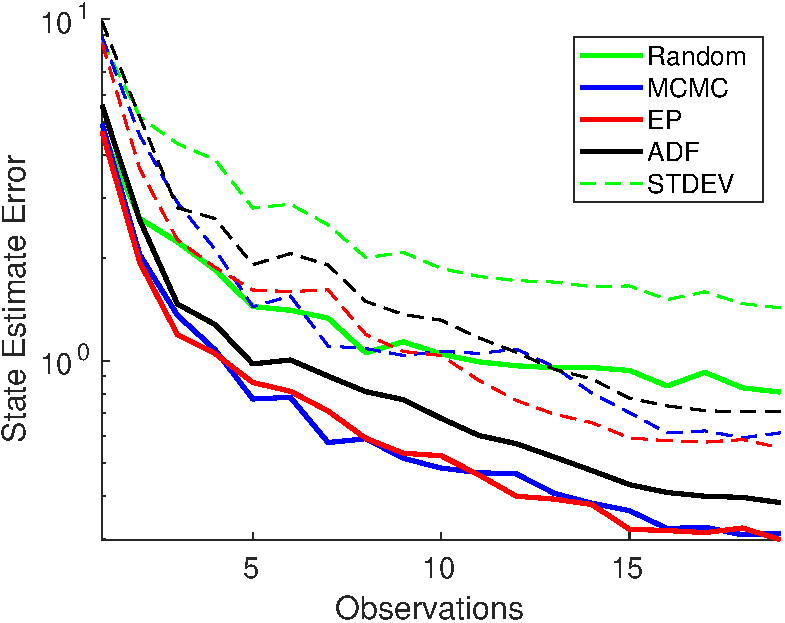
\includegraphics[width=0.24\textwidth]{ss_stateerr} &
    \hspace{-5mm}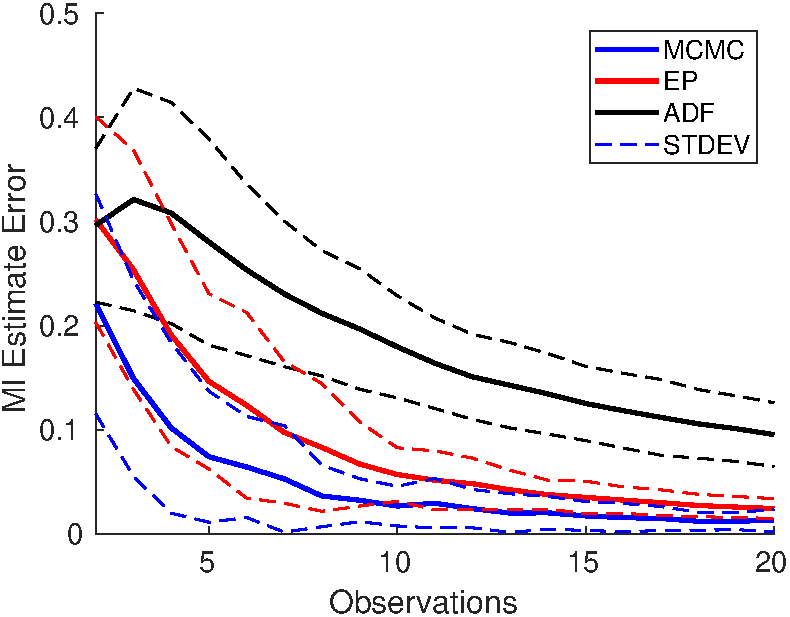
\includegraphics[width=0.24\textwidth]{ss_MIerr}
  \end{tabular}
  
  \caption{\small\textbf{Static target estimation.} Estimation of a 1D
    target position in a network of $K=10$ equally spaced
    sensors.  \emph{Left:} Variational planning based on EP inference
    yields comparable error in state estimate compared to MC
    estimation with 50 samples. ADF inference yields higher error.
    All methods outperform random selection.  \emph{Right:} MC
    estimation produces the most accure MI estimates as compared to
    numerical calculation, whereas ADF yields higher error due to
    increased bound gap.}
  \label{fig:static}
\end{figure}

We optimize the MI lower bound over a linear Gaussian $\omega(x \mid
y_t) = \Ncal(Cx,\nu^2)$, which can be solved in closed-form.  To
compare the impact of inference on planning we consider MCMC, EP and
assumed density filtering (ADF).  As shown in \FIG\ref{fig:static} we
find that quality of the posterior approximation impacts quality of
both the state estimate (\emph{left}) and selected actions
(\emph{right}).  While ADF is more computationally efficient and
numerically stable than EP, it tends to produce less accurate
posterior estimates.  Variational planning based on the EP posterior
yields state estimates on-par with MCMC, though the latter produces
better quality MI estimates in this low-dimensional example.

\subsubsection{Dynamical System}

Extending the above analysis to a dynamical system with, we consider a
nonlinear dynamics frequently used in the sequential Monte Carlo
literature~\citep{kitagawa1996monte, gordon1993novel,
cappe2007overview},
\[
  \Ncal\left(0.5 x_{t-1} + 25 x_{t-1} / (1+x_{t-1}^2)
  + 8 \cos(1.2t), \sigma_u^2\right).
\]
Observations are again drawn from one of $K=10$ sensors at each time
with nonlinear Gaussian noise,
\[
  y_t \mid x_t; k \sim \Ncal(x_t^2/20, v_{tk}(x_t))
\]
with variance $v_{tk}(x_t)$ identical to the preceding example.
Continuing our analysis of the static case, we compare exact inference
with a particle filter under, both, variational and Monte Carlo
planning strategies.

Results in \FIG\ref{fig:dynamic} report squared error of the state
estimate, relative to truth, and squared error of the selected sensor
relative to the sensor closest to the target.  The latter is
a reasonable baseline since sensor noise is driven by relative
distance.  While exact inference with variational planning is best
overall, we find comparable planning results between Monte Carlo
estimation (MCMI) and variational when particle filter inference is
used.

\begin{figure}
  \begin{tabular}{cc}
    \hspace{-3mm}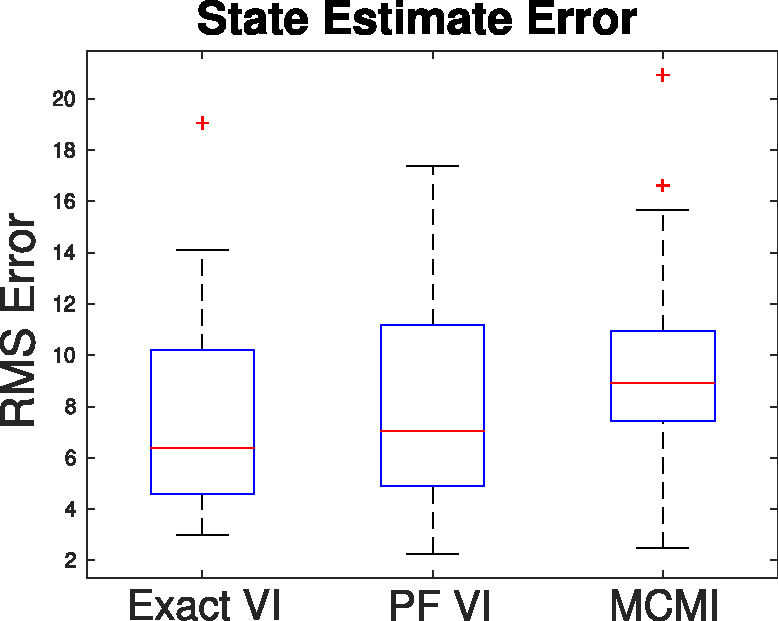
\includegraphics[width=0.23\textwidth]{tracking_state_err} &
    \hspace{-3mm}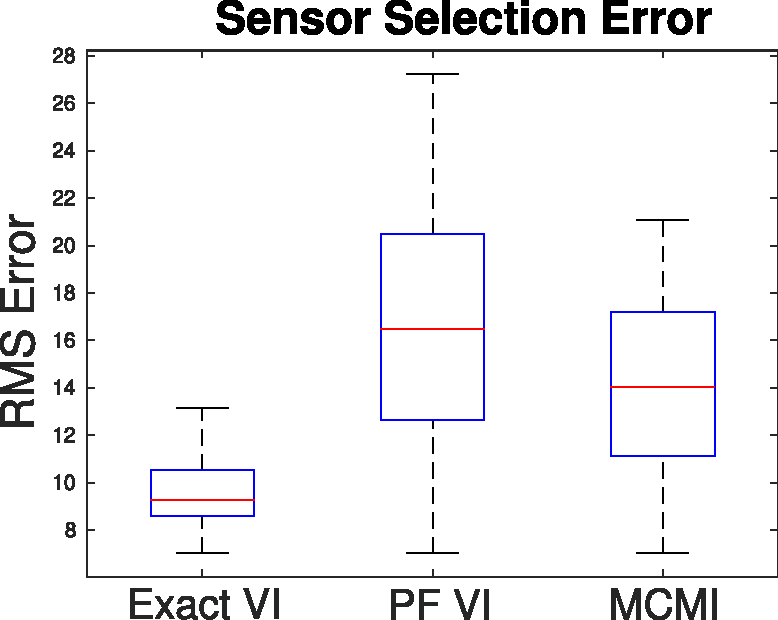
\includegraphics[width=0.23\textwidth]{tracking_sensor_err}
  \end{tabular}
  
  \caption{\small\textbf{Nonlinear tracking for 20 random
  trials.}  \emph{Left:} Exact inference with variational planning
  yields the lowest RMS state error.  Particle filter inference with
  500 particles and variational planning (PFVI) yields lower median
  error compared to MC estimates of information (MCMI), though wider
  error quantiles.  \emph{Right:} Again, Exact VI shows the lowest RMS
  error of the selected sensor position w.r.t.~optimal, whereas PFVI
  and MCMI both have higher error, again with PFVI having larger
  quantiles.}
  \label{fig:dynamic}
\end{figure}


\begin{figure*}[!t]
  \centering
  \hspace{-3mm}
  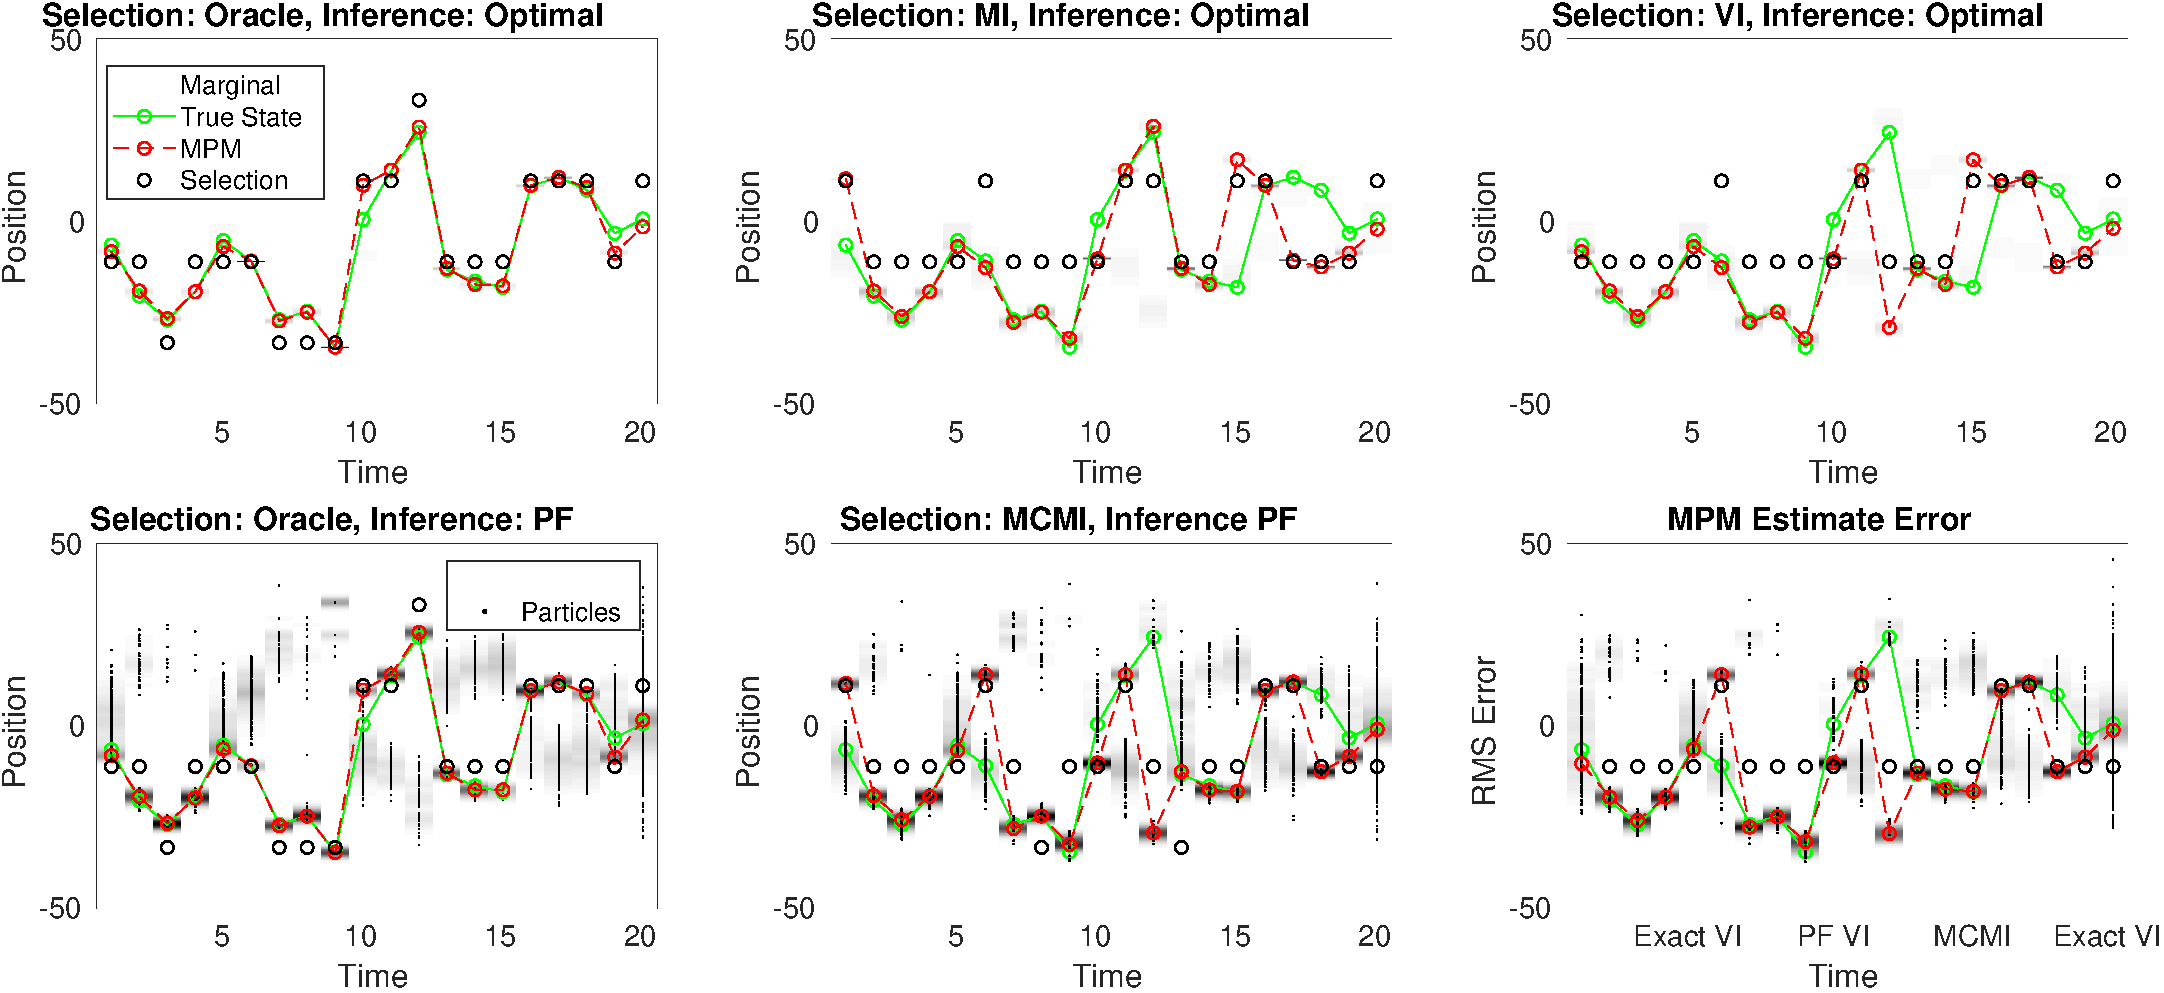
\includegraphics[width=0.9\textwidth]{tracking_single}
  \vspace{-3mm}
  \caption{\small\textbf{Nonlinear state-space example.} Random instance
    showing estimates for various inference and planning methods.}
  \label{fig:ep}
\end{figure*}



\subsection{Gene Regulatory Network}
\RED{I will likely push this experiment into a supplement. Results do
  not show a strong improvement over the previously published
  approach.}

Next, we adopt the sparse linear model considered
by~\cite{steinke2007experimental} and~\cite{seeger2008bayesian} to
demonstrate variational planning for inferring gene regulatory
networks.  Let $x\in\RR^n$ represent the deviation of gene expression
levels from steady state for $n=50$ genes.  The matrix
$A\in\RR^{n\times n}$ represents a directed network of interactions,
with sparse entries drawn independently from a Laplace distribution.
\begin{equation}\label{eq:sparselin}
  \!\!\!p(A,x) \propto \prod_{i=1}^n \Ncal(u_i \mid a_i^T
    x, \sigma^2) \prod_{j=1}^n \textrm{Laplace}(a_{ij} \mid \lambda) 
\end{equation}
where $a_i$ is the $i^{\text{th}}$ row of matrix $A$.  Here $u$
represents an external control vector (perturbation). Observe that the
joint~\eqref{eq:sparselin} is defined up to normalization since the
likelihood term is not a normalized distribution of $x$.

\begin{figure}
  \centering
  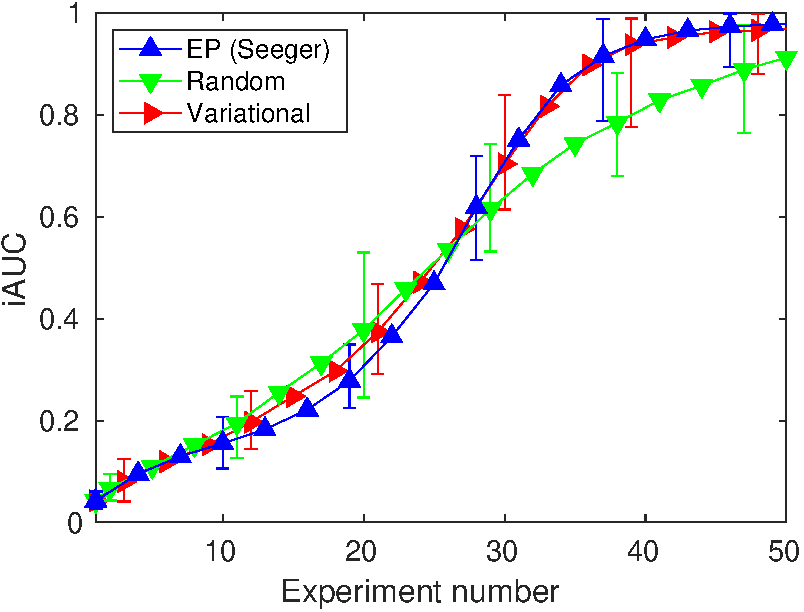
\includegraphics[width=0.35\textwidth]{sparselin_iAUC_N100_norandom_run20_norepeats}
  \caption{\small\textbf{Sparse linear model.} Area under the curve
  for true edges with weights $|a_{ij}|>0.1$ plotted for each
  intervention experiment.  Variational planning shows moderate
  improvement over~\citep{seeger2008bayesian} for less than 25
  experiments, and is on par thereafter.}
  \label{fig:sparselin}
\end{figure}

We use the EP implementation provided by~\cite{seeger2008bayesian},
which maintains a mean field Gaussian posterior
approximation, \mbox{$q(A) = \prod_i
p_i^{(0)}(a_i) \prod_j \widetilde{t}_{ij}(a_{ij})$}.  Here,
$p^{(0)}_i(a_i)$ approximates the base measure \mbox{$N(u_i \mid a_i^T
x, \sigma^2)$} and \mbox{$\widetilde{t}_{ij}(a_{ij})$} approximate Laplace
factors.

The previous authors introduce a planning heuristic by noting that,
given a control and corresponding observation $\{x_*,u_*\}$,
maximizing MI is equivalent to,
\begin{equation}\label{eq:max_kl}
  \max_{u_*} \; \EE_{x_*}\!\left[\, \KL{q'}{q} \,\right].
\end{equation}
Here $q'(A) \approx p(A \mid D \cup \{x_*,u_*\})$ is the posterior
approximation with inclusion of the new data.  Expectation is over the
approximate posterior predictive distribution, which cannot be
expressed in closed form, but can be sampled.
Computing~\eqref{eq:max_kl} requires full updates to the EP posterior
for each data sample, which is prohibitive.  The authors instead
propose to only update the base measure $p^{(0)}$.

%% which matches
%% moments of $q^{'}$ to those of.  Specifically, the
%% augmented distribution is given by,
%% \[
%%   \hat{p}(a_i, x_*) \propto \Ncal(u_* \mid a_i^T
%%   x_*, \sigma^2) \prod_j \widetilde{t}_{ij}(a_{ij}).
%% \]
%% The EP update then matches moments to the augmented distribution above
%% for each row $a_i$.
%% %% $\EE_{\hat{p}}[a_i] = \EE_{q'}[ a_i ]$ and $\text{var}_{\hat{p}}[ a_i
%% %% ] = \text{var}_{q'}[ a_i ]$ for each row $a_i$.
%% %% \[
%% %%   q' \Leftrightarrow \argmin_{q'} \KL{}{q'}
%% %% \]

We demonstrate our approach for 20 random networks, each with $n=50$
nodes.  The variational MI bound is optimized in closed-form for a
linear Gaussian approximation $\omega(a_i \mid x)
= \Ncal(Fx, \lambda^2 I)$ on each row.  Following the original
analysis, we present results using a variation of area under the curve
(iAUC) which scores prediction of \emph{strong} edges, specifically
those with true weight $|a_{ij}| > 0.1$.

prediction results in \FIG\ref{fig:sparselin}

\subsection{Labeled LDA}\label{sec:llda}

%% \begin{figure*}
%%   \begin{minipage}{0.4\textwidth}
%%     \includegraphics[width=1.0\textwidth]{llda_tverr}
%%   \end{minipage}
%%   \begin{minipage}{0.6\textwidth}
%%     \begin{tabular}{cccc}
%%       \hspace{-8mm}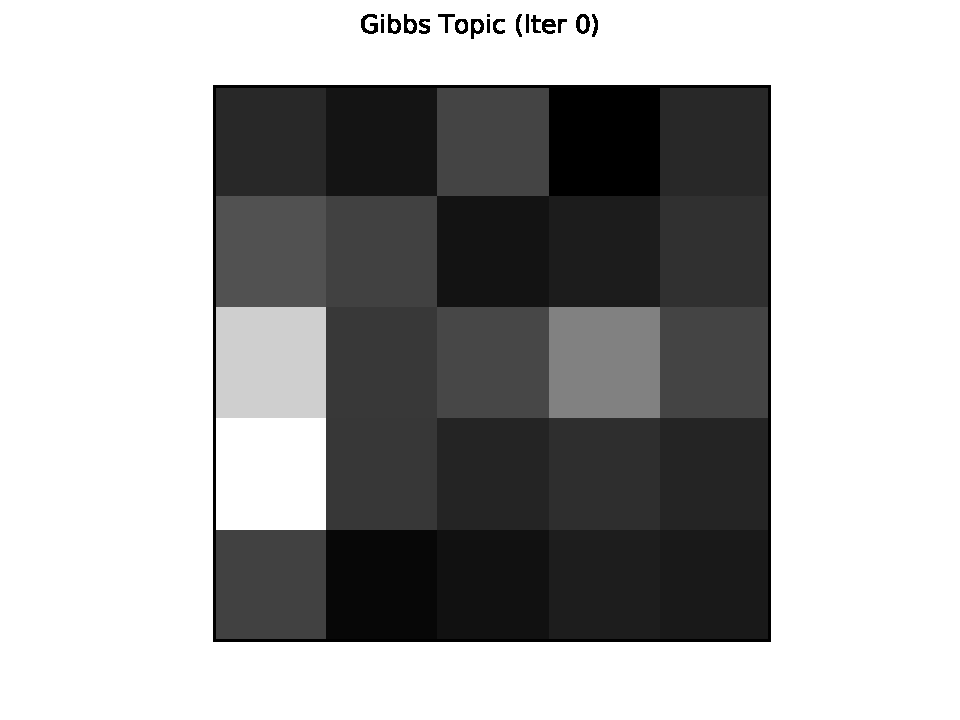
\includegraphics[width=0.35\textwidth]{llda/Gibbs_iter0} &
%%       \hspace{-12mm}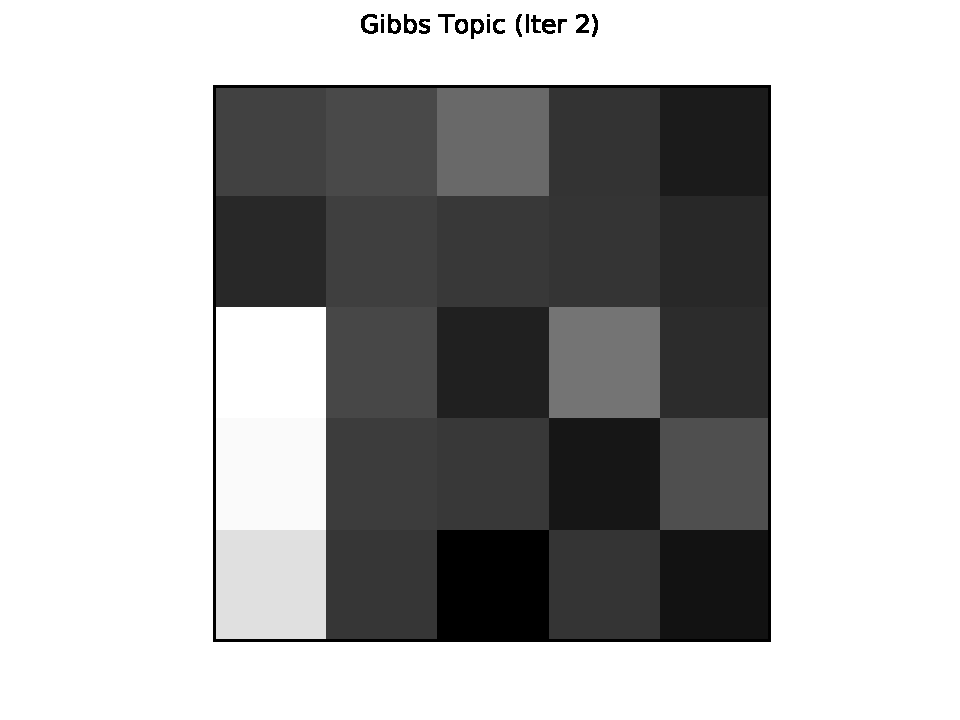
\includegraphics[width=0.35\textwidth]{llda/Gibbs_iter2} &
%%       \hspace{-12mm}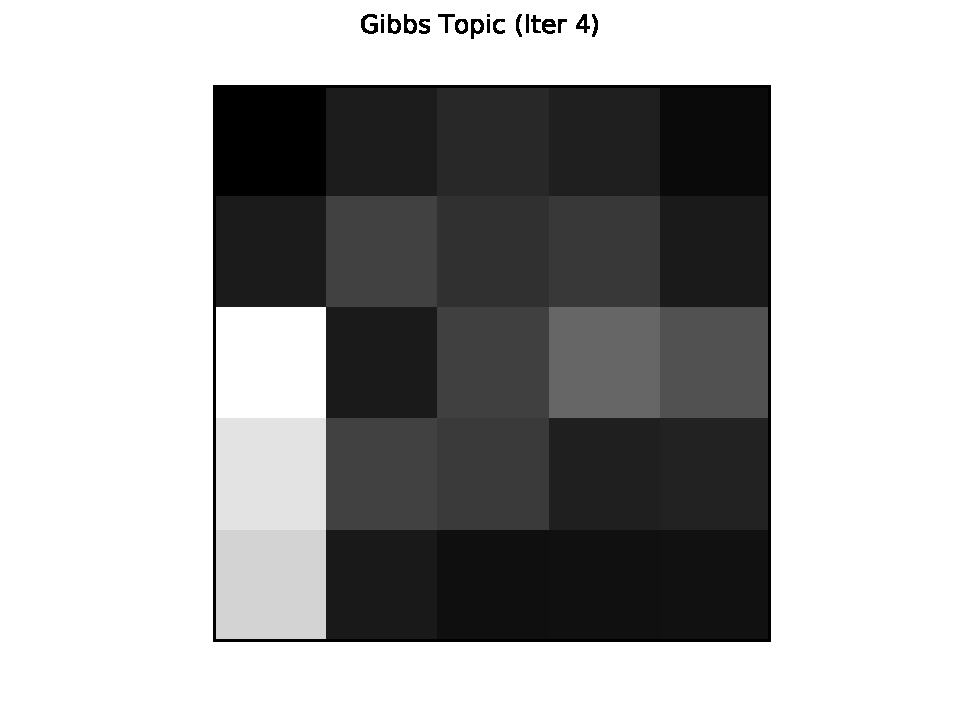
\includegraphics[width=0.35\textwidth]{llda/Gibbs_iter4} &
%%       \hspace{-12mm}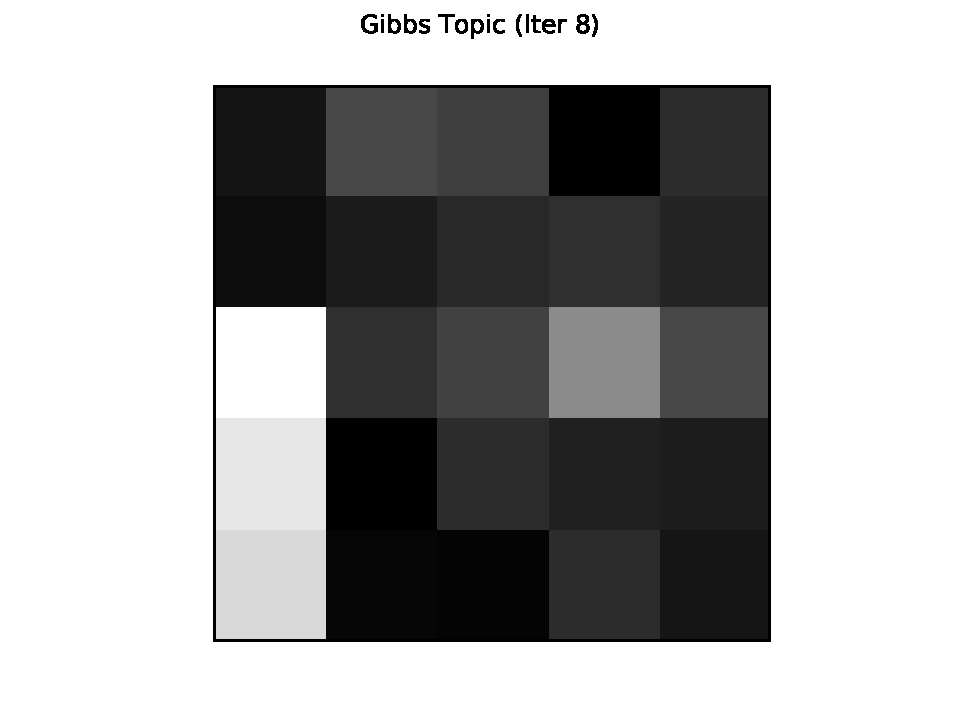
\includegraphics[width=0.35\textwidth]{llda/Gibbs_iter8} \\
      
%%       \hspace{-8mm}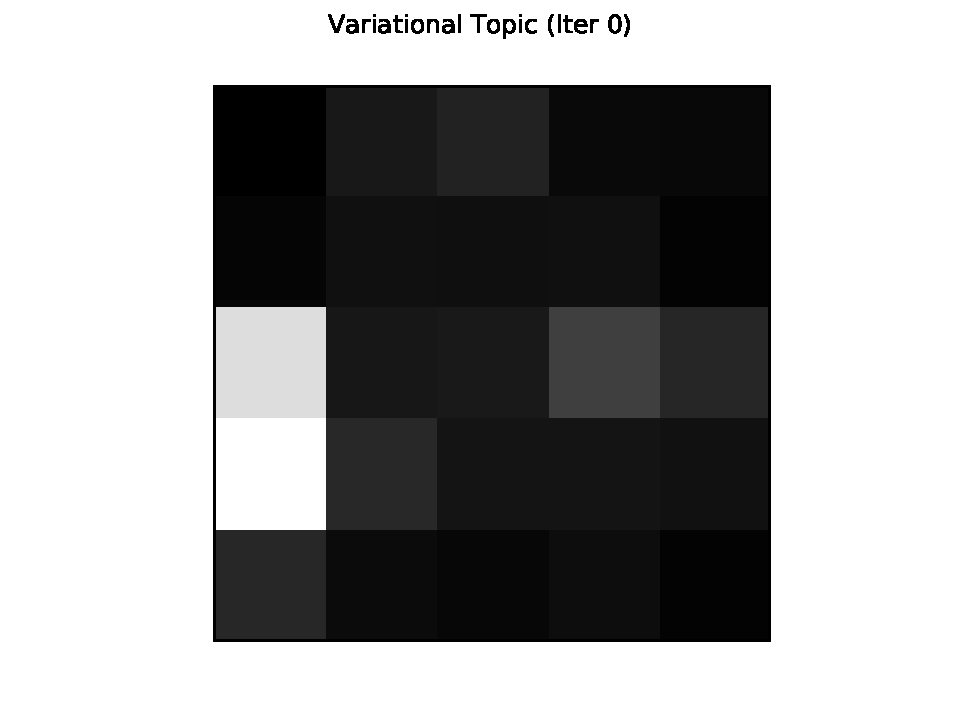
\includegraphics[width=0.35\textwidth]{llda/Variational_iter0} &
%%       \hspace{-12mm}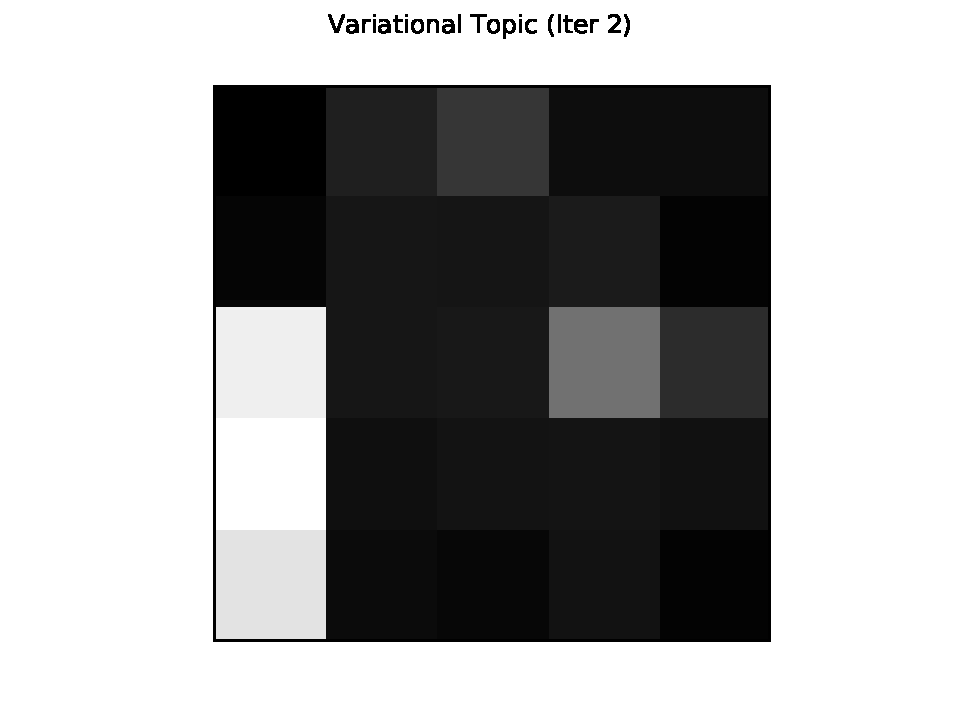
\includegraphics[width=0.35\textwidth]{llda/Variational_iter2} &
%%       \hspace{-12mm}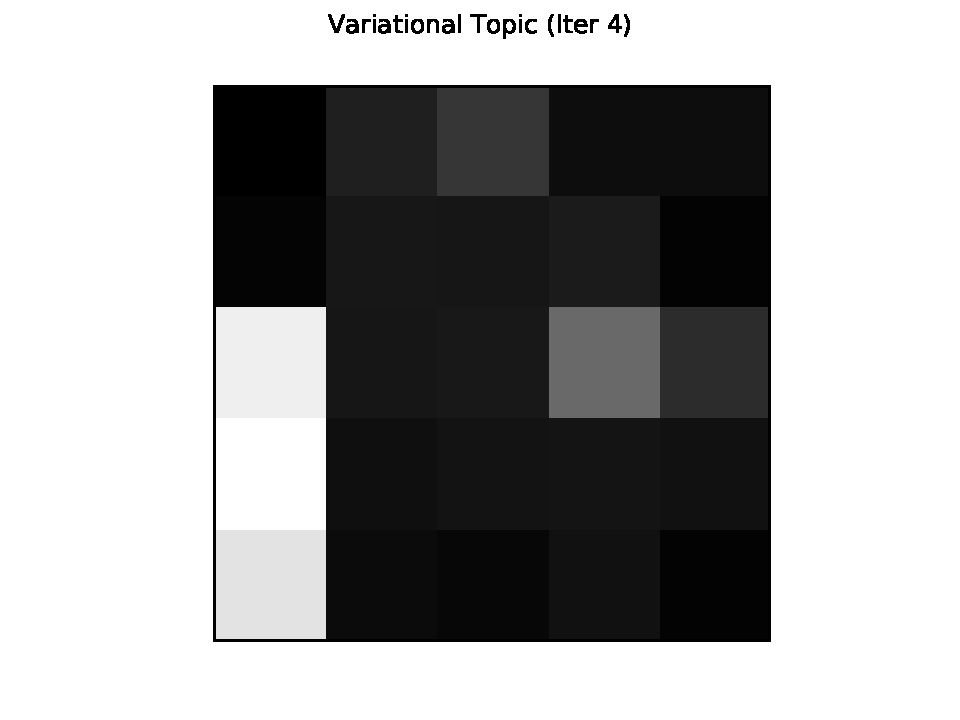
\includegraphics[width=0.35\textwidth]{llda/Variational_iter4} &
%%       \hspace{-12mm}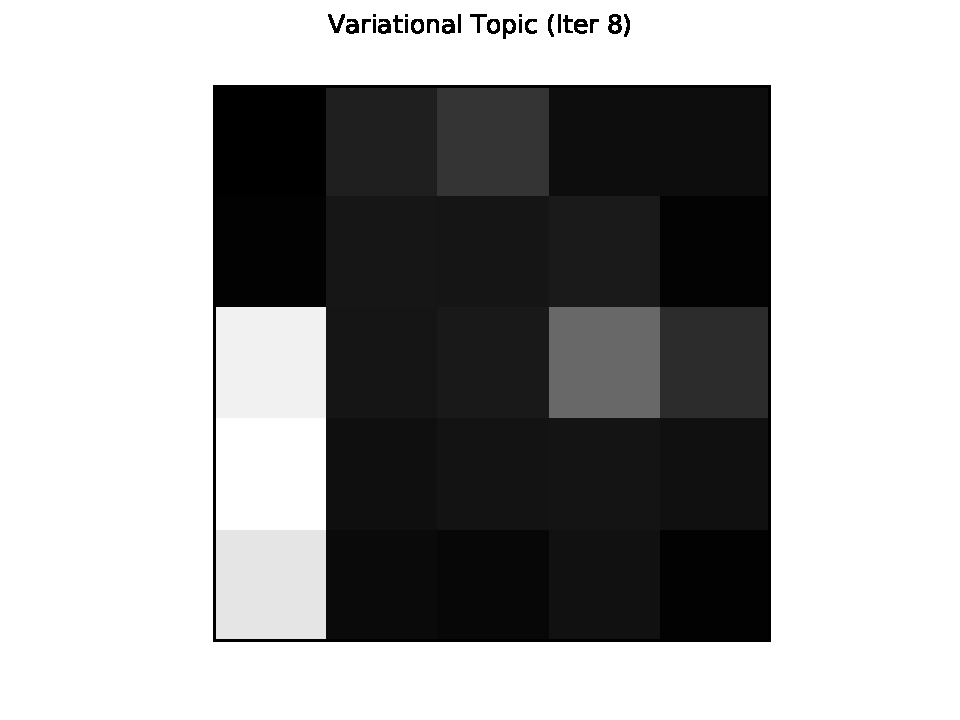
\includegraphics[width=0.35\textwidth]{llda/Variational_iter8}
%%     \end{tabular}
%%   \end{minipage}
%%   \caption{\small\textbf{Labeled LDA.} Blah.}
%% \end{figure*}

\begin{figure}
  \centering
  \includegraphics[width=0.45\textwidth]{llda/llda_tverr} \vspace{-2mm}
  
  \caption{\small\textbf{Labeled LDA.} Total variation error (absolute
  error) for all topics on the ``bars'' dataset across 10 random
  trials.  Variational planning with fully parameterized softmax shows
  consistent improvement over Gibbs on average (solid).  Gibbs
  estimates show tighter standard deviation (shaded) for planning
  based on MI estimates.  Both inference methods perform similarly
  for random selection.}
  
  \label{fig:llda_tv}
\end{figure}

\begin{figure}
  \centering
  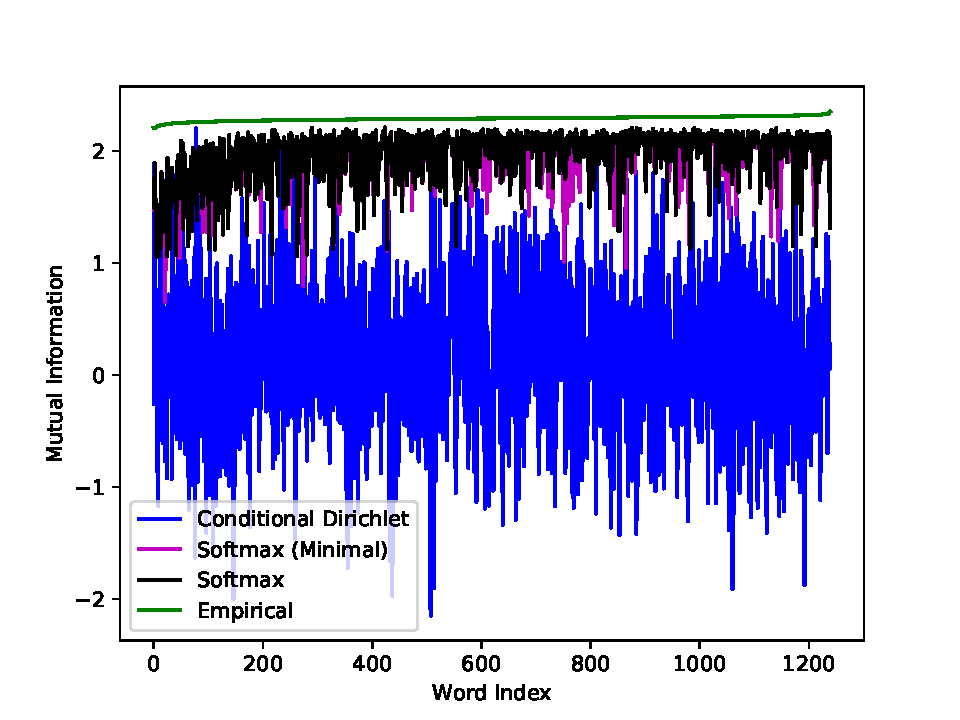
\includegraphics[width=0.45\textwidth]{llda/bound_comparison}
  
  \caption{\small\textbf{LLDA Bound Comparison.} Variational MI
  estimates for annotations using three approximating families, ranked
  in order of increasing value by empirical estimate of MI.  An ideal
  approximation would show monotonically increasing values with little
  gap.  The conditional Dirichlet model is a poor approximation.  Two
  variations on the softmax distribution provide tighter bounds, with
  the fully parameterized softmax being slightly
  preferred.}  \label{fig:llda_bound}
\end{figure}

Labeled LDA (LLDA) is one of several proposed semi-supervised
extensions to LDA~\citep{blei2003latent}.  The standard unsupervised
LDA model is given by,
\begin{align*}
  \theta_d &\sim \text{Dirichlet}(\alpha), &&\text{For}\; d=1,\ldots,D \\
  \psi_k &\sim \text{Dirichlet}(\beta_k), &&\text{For}\; k=1,\ldots,K \\
  z_{dn} \mid \theta_d &\sim \text{Cat}(\theta_d), &&\text{For}\;
    n=1,\ldots,N_d \\
  w_{dn} \mid z_{dn}, \psi &\sim \text{Cat}(\psi_{z_{dn}}) &&
\end{align*}
In addition, LLDA as proposed in~\cite{flaherty2005latent} augments
the model with semi-supervised annotations for each word.  We model
annotations as noisy observations of the true topic assignment:
$y_{dn} \mid z_{dn} \sim \text{Cat}(\pi_{z_{dn}})$.  In this way,
annotations induce a preferred ordering of topic labels in the posterior.

We demonstrate our approach on the ``bars''
dataset~\citep{griffiths2004finding}.  Using a vocabulary of $W=25$
words, each of the $K=10$ topics places the majority of mass on a
single column / row when visualized as $5\times 5$ images. The planner
selects an annotation $y_{d^*n^*}$ maximizing MI of the
topics,
\begin{equation}
  (d^*,n^*) = \argmax_{(d,n)} I(\Psi, Y_{dn}).
\end{equation}
We demonstrate information theoretic active learning on a corpus of
$D=50$ documents, each with $N_d=25$ words.  We model a \emph{rare}
topic by setting a non-symmetric Dirichlet prior on topic proportions:
$\alpha = (0.05, 1, 1, \ldots, 1)^T$.  A planner should prefer
annotations for words likely to arise from this rare topic.

\textbf{Lower topic error compared to Monte Carlo.}
\FIG\ref{fig:llda_tv} reports total variation (TV) error across topics
$\sum_k \|\psi_k - \hat{\psi}_k\|_1$, based on the posterior mean
estimate $\hat{\psi}$.  To account for topic label differences we
solve a bipartite matching to compute the lowest TV error across
labels.  Increasing MCMC samples from the reported 1000 does not lead
to significant improvements.  We instead suspect that poor MCMC
results are due to a combination of MI estimator bias, inference local
optima, and topic label switching.

\textbf{Topic label switching.}
Empirical MI estimates based on Gibbs samples involve averages across
independent MCMC chains, and are thus sensitive to topic label
switching~\citep{stephens2000dealing}.  We found that alignment to the
MAP sample, or indeed any individual sample, produced poor results.
We instead relabel samples to minimize the total variation (TV) error
w.r.t.~the ground truth topics.  Such an approach would not be
possible in typical cases as it requires knowledge of the true topics.
Our variational planning approach does not suffer similar issues as
samples are drawn from a consistent topic posterior distribution.

\textbf{More flexible approximations lead to better bounds.}
We begin by exploring the impact of different approximating families
on the variational MI bound.  \FIG\ref{fig:llda_bound} compares
variational MI estimates to that of an empirical estimate for three
approximating families: a conditional Dirichlet, $\omega(\psi \mid
y=j) = \prod_k \text{Dirichlet}(\psi_k \mid \gamma_{kj})$,
a \emph{minimal} softmax where class conditionals depend on a single
topic $\omega(y = k \mid \psi) \propto \exp( w_k^T \text{vec}(\psi_k)
+ w_{0k} )$, and where class conditionals weight all topics
$\omega(y = k \mid \psi) \propto \exp( w_k^T \text{vec}(\psi) + w_{0k}
)$.  We find that the larger parameter set of this final family leads
to more accurate bounds overall.


%% MI as $I(\Psi,Y_{dn}) \geq H(Y_{dn})
%% + \EE[ \log \omega(Y_{dn} \mid \Psi) ]$ using the following softmax
%% distribution,
%% \begin{equation}
%%   \omega(Y = k \mid \Psi) \propto \exp( w_k^T \text{vec}(\Psi) +
%%   w_{0k} ).
%% \end{equation}

%% which is in the exponential family with natural parameters
%% $\theta(\Psi) = (w_1^T \text{vec}(\Psi) + w_{01}, \ldots,
%% w_K^T \text{vec} + w_{0K})^T$.





